\documentclass[12pt,a4paper,danish]{article}
\usepackage[ansinew]{inputenc}
\usepackage{amsmath}
\usepackage{amsfonts}
\usepackage{amssymb}
\usepackage{graphicx}
\author{Gruppe 5}
\title{Databaser - Hand In 1} 
\begin{document}
\maketitle
\pagebreak
\subsection*{Indledning}
Dette dokument beskriver, hvordan gruppen er kommet frem til det vedlagte databasediagram, samt de queries, der er blevet skrevet. Hertil er der blevet gjort brug af CRUD-operationerne (\textbf{C}reate, \textbf{R}ead, \textbf{U}pdate og \textbf{D}elete).\\\\
Til denne opgave skulle der skabes tre components. En System Log component til at logge systemevents, en Inventory component til at holde data fra dele af systemet, samt en Converting component til udregne data for de forskellige klodser og placerer dem efter dette.

\subsection*{Process}
\subsubsection*{F�rste del: OO UC diagram}
Use Case diagrammerne er delt op i de overn�vnte komponenter og kan ses nedenfor:
\begin{figure}[h]
\centering
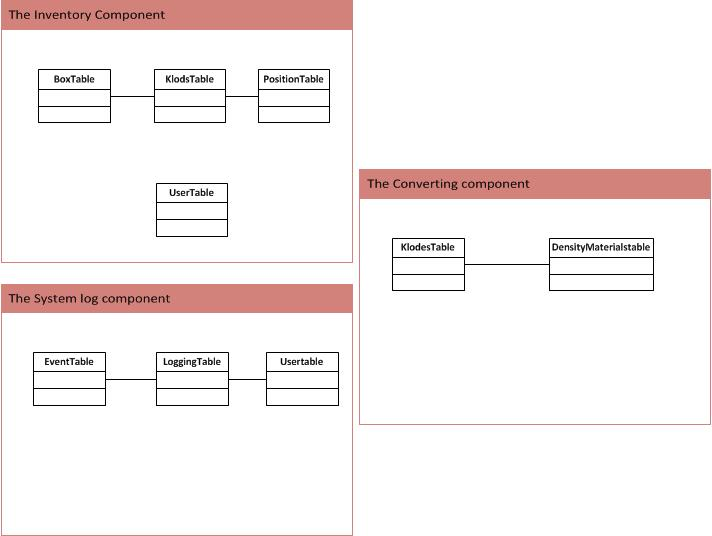
\includegraphics[scale=0.7]{../../Diagrammer/Klassediagrammer/Database/DatabaseUML.jpg}
\caption{UML diagram over Databaser}
\end{figure}\\
\textbf{The Inventory Component}\\
Dette komponent best�r af \textit{BoxTable}, \textit{KlodsTable}, \textit{PositionTable} og \textit{UserTable}. \textit{BoxTable} har til ansvar at holde styr p�, hvilke og hvor mange klodser der kan l�gges i boksens r�kker og kolonner. \\\textit{KlodsTable} har til ansvar at holde styr p� data i henhold til den specifikke klods. Det er bl.a. parametre som klodsens masse, rumfang, l�ngder og densitet der bliver holdt styr p�. \\ \textit{PositionTable} best�r af koordinater til boksen, samt hvilke r�kke og kolonner der kan ligges noget i.\\ \textit{UserTables} ansvar er at holde styr p� BrugerId og password samt tilh�rende privilegier. \\\\
\textbf{The Converting Componement}\\
Dette komponent best�r af en \textit{klodsTable} og en \textit{densityMaterialsTable}.\\
\\ \textit{KlodsTable} ansvar er det samme som i overn�vnte afsnit. \\ \textit{DensityMaterialsTable} har til ansvar at sammenligne den specifikke klods' udregnede densitet med en tabel over densiteter for forskellige materialer. \\\\
\textbf{The System Log Componement}\\
Dette komponent best�r af \textit{EventTable}, \textit{LoggingTable} og \textit{UserTable}.\\ \\\textit{EventTables} ansvar er at logge systemets status hvis der sker fejl, samt tilh�rende fejlkoder. \\\textit{LoggingTable} ansvar er at give tidspunkter for hvorn�r den valgte h�ndelse skete. \\\textit{UserTable} er beskrevet ovenfor og har samme ansvar her. 

\newpage
\subsubsection*{Anden del: Database diagram}
Billedet nedenfor viser en oversigt over Databasen, med tilh�rende tabeller og attributter:
\begin{figure}[h]
\centering
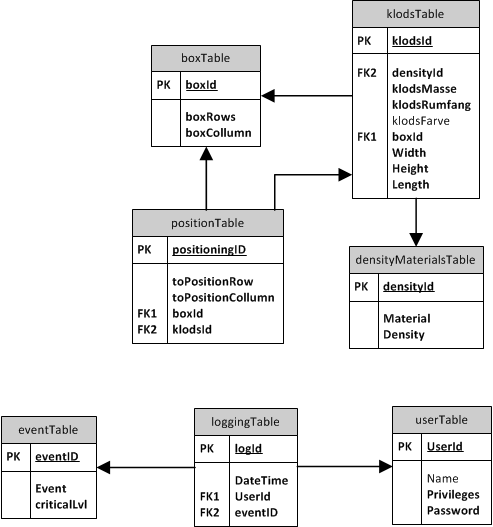
\includegraphics[scale=0.7]{../../Diagrammer/Klassediagrammer/Database/databaseDiagramPic.png}
\caption{Database Diagram}
\end{figure}\\

\textbf{Keys}
Ved hver table er der som bekendt en primary key (og en foreign key, som her blot er primary key'en fra en anden table). Her f�lger en beskrivelse af hver key til hver table
\begin{enumerate}
\item loggingTable
	\begin{itemize}
	\item LogId - Denne n�gle bliver ikke brugt til andet, end at give hvert log indl�g et nummer. Dette 					  nummer inkrementeres med �n ved hvert log event.
	\end{itemize}
\item eventTable
	\begin{itemize}
	\item eventId - Alle log events er beskrevet i dette table. Denne key beskriver hvilken event 						afdeling samt hvilket event der er forekommet(eg. Nummer 47 ligger i afdelingen 1-50, 					som er �n type events). 
	\end{itemize}
\item userTable
	\begin{itemize}
	\item brugerId - Beskriver en specifik bruger. Denne bruger har brugernavn, privilegier og et 								 password
	\end{itemize}
\item klodsTable
	\begin{itemize}
	\item klodsId - N�r en ny klods identificeres af systemet, gemmes dens data med et nyt klodsId. Dette 					id er n�glen
	\end{itemize}
\item densityMaterialTable
	\begin{itemize}
	\item densityId - En lang liste af materialer med tilh�rende densitet. I tilf�lde af, at der kommer 						  en klods, der har en densitet der ikke eksisterer i tabellen, vil den f� en ny key 						  og et	navn.
	\end{itemize}
\item boxTable
	\begin{itemize}
	\item boxId - Beskriver hvilken boks der bruges, i tilf�lde af flere bokse
	\end{itemize}
\item positionTable
	\begin{itemize}
	\item positionId - Alle positioner, der er i en given boks
	\end{itemize}
\end{enumerate}

\end{document} 